\chapter{Recurrence}

\section{Linear Recurrence}

\begin{definition}
    A recurrence is called \textbf{linear} when there are $k \geq 1$ constants $c_0, \cdots ,c_k \in \R$ and $g:\Z \rightarrow \R$ such that
    $$c_ka_{n+k}+ \cdots +c_0a_n=g(n)$$
\end{definition}
\noindent \textbf{Example}: $5a_{n+1}-a_n=n^2$ is a linear recurrence.

\begin{definition}
    A recurrence is called \textbf{homogeneous} if it only depends on previous terms of the sequence. 
    In the case of a linear recurrence this means that there is a $k \geq 1$ and constants $c_0, \cdots ,c_k \in \R$ such that 
    $$c_ka_{n+k}+ \cdots +c_0a_n=0$$
\end{definition}


\section{Advancement Operator}
\begin{definition}
    Now for sequence $a_n$, we will simply write the shorthand $\vec{a}$
\end{definition}
\textbf{Remark}:
\begin{itemize}
    \item We can view a sequence as an infinite dimensional vector.
\end{itemize}

\begin{definition}
    The \textbf{advancement operator} $A$ is a function that maps sequences to sequences defined by:
    $$A\vec{a}=\vec{b} \text{ where } b_n=a_{n+1}$$
    We write $A^k$ as a shorthand for k-compositions of $A$ and take $A^0$ to be the identity map $A^0\vec{a}=\vec{a}$
\end{definition}
\noindent \textbf{Example}: Recall the backward shift operator $T \in \mathcal{L}(\mathbb{F}^{\infty})$ defined by $T(z_1,z_2,z_3, \cdots)=(z_2,z_3, \cdots)$ that we talked in MAT240.

\begin{definition}
    Given a sequence $\vec{a}$ and a constant $c \in \R$, we let $c \cdot \vec{a}$ denote the sequence $ca_n$. 
    We also define the sum of two sequences $\vec{a}+\vec{b}$ to be the sequence $a_n+b_n$.
\end{definition}

\begin{lemma}
    For any sequence $\vec{a}$ and any constant $c \in \R$. $$A(c \cdot \vec{a})=c \cdot A\vec{a}$$
\end{lemma}

\begin{lemma}
    For any pair of sequnces $\vec{a}$ and $\vec{b}$. $$A(\vec{a}+\vec{b})=A\vec{a}+A\vec{b}$$
\end{lemma}

\begin{theorem}[The first advancement theorem]
    Let $r \in \R$.
    $$(A-r)\vec{a}=0 \text{ iff } \exists \alpha \in \R. \forall n \in \N. a_n=\alpha r^n$$
\end{theorem}
\textbf{Remark}
\begin{itemize}
    \item $(A-r)\vec{a}=o$ is equivalent to $a_n$ is a geometric progression with common ratio $r$.
\end{itemize}
\begin{proof}
    $(A-r)\vec{a}=A\vec{a}-r\vec{a}$ which is the sequence $a_{n+1}-ra_n$\\
    $(\Rightarrow)$\\
    Suppose we have a sequence $a_n$ and $a_{n+1}-ra_n=0$. 
    We can show by induction that $a_n=a_0 \cdot r^n$.\\
    $(\Leftarrow)$\\
    Consider the sequence $a_n=\alpha \cdot r^n$, then $a_{n+1}-ra_n=\alpha r^{n+1}- \alpha r^{n+1}=0$ as desired.
\end{proof}

\begin{definition}
    Let $p(x)=\sum_{i=0}^{k}c_ix^i$ be a polynomial. We have $p(A)\vec{a}=\sum_{i=0}^{k}c_iA^i\vec{a}$
\end{definition}

\begin{lemma}
    Let $p(x)=\sum_{i=0}^{k}c_ix^i$,\\
    $p(X)\vec{a}=\vec{b}$ iff the sequence $\vec{a}$ satisfies the linear recurrence $\sum_{i=0}^kc_ia_{n+i}=b_n$.
\end{lemma}

\begin{theorem}[Advancement factorization]
    Let $p(x)=\sum_{i=0}^kc_ix^i$ and suppose there is a polynomial $q(x)=\sum_{i=0}^{k-1}d_ix^i$ and a real number $r \in \R$ such that $p(x)=(x-r)q(x)$. 
    We then have the advancement equation:
    $$p(A)\vec{a}=(A-r)(q(A)\vec{a})=q(A)((A-r)\vec{a})$$
\end{theorem}
\begin{proof}
    $p(x)$ can be represented in another way:
    \begin{equation}
        \begin{split}
            p(x) &= (x-r)q(x)\\
            &= xq(x)-rq(x)\\
            &= \sum_{i=0}^{k-1}d_ix^{i+1}-\sum_{i=0}^{k-1}rd_ix^i
        \end{split}
    \end{equation}
    \begin{equation}
        \begin{split}
            (A-r)(q(A)\vec{a}) &= (A-r)(\sum_{i=0}^{k-1}d_iA^i\vec{a})\\
            &= A(\sum_{i=0}^{k-1}d_iA^i\vec{a})-r(\sum_{i=0}^{k-1}d_iA^i\vec{a})\\
            &= \sum_{i=0}^{k-1}d_iA^{i+1}\vec{a}-\sum_{i=0}^{k-1}rd_iA^i\vec{a}\\
            &= p(A)\vec{a}
        \end{split}
    \end{equation}
\end{proof}

\noindent \underline{Zero is our hero.}

\begin{lemma}
    Let $p(x)$ be a polynomial.\\
    If $p(A)\vec{x}=\vec{b}$ and $p(A)\vec{y}=\vec{b}$, then $p(A)(\vec{x}-\vec{y})=0$.
\end{lemma}
\begin{proof}
    \begin{equation}
        \begin{split}
            p(A)(\vec{x}-\vec{y}) &= p(A)\vec{x}-p(A)\vec{y}\\
            &= \vec{b}-\vec{b}\\
            &= 0
        \end{split}
    \end{equation}
\end{proof}

\noindent Actually, we have a strengthend version of the first advancement theorem.
\begin{theorem}[The principle theorem]
    Suppose $p(x)=\prod_{i=1}^k(x-r_i)$ where the $r_i$ are distinct.\\
    It follows that $p(A)\vec{a}=0$ iff $\exists \alpha_1, \cdots \alpha_k.a_n=\sum_{i=1}^k\alpha_ir_i^n$
\end{theorem}
\begin{proof}
    $(\Leftarrow)$\\
    Assume $a_n=\sum_{i=1}^k\alpha_ir_i^n$\\
    We notice that 
    \begin{equation}
        \begin{split}
            (A-c)\vec{a} &= A\vec{a}-c\vec{a}\\
            &= a_{n+1}-ca_n\\
            &= \sum_{i=1}^k\alpha_ir_i^{n+1}-c\sum_{i=1}^k\alpha_ir_i^n\\
            &= \sum_{i=1}^k\alpha_i(r_i-c)r_i^n
        \end{split}
    \end{equation}
    $(A-c)$ can be viewed as an operator that sends sequences of the form $\sum_{i=1}^kx_ir_i^n$ to \\$\sum_{i=1}^k\alpha_i(r_i-c)r_i^n$\\
    \begin{equation}
        \begin{split}
            p(A)\vec{a} &= (A-r_1)(A-r_2)\cdots(A-r_k)\vec{a}\\
            &= (A-r_1)(A-r_2)\cdots(A-r_{k-1})(\sum_{i=1}^k\alpha_i(r_i-r_k)r_i^n)\\
            &= (A-r_1)(A-r_2)\cdots(A-r_{k-2})(\sum_{i=1}^k\alpha_i(r_i-r_k)(r_i-r_{k-1})r_i^n)\\
            &= \sum_{i=1}^k\alpha_i(\prod_{j=1}^k(r_i-r_j)r_i^n)\\
            &= 0
        \end{split}
    \end{equation}
    $(\Leftarrow)$ Induction on $k$.\\
    Base case: \\
    $k=1$. By the first advancement theorem, the claim is true.\\
    Inductive step:\\
    Assume the claim is true for $k$.\\
    Suppose $p(x)=\prod_{i=1}^k(x-r_i)$ where $r_i$ are distinct. \\
    And $p(A)\vec{a}=0 \Rightarrow \exists\alpha_1, \cdots ,\alpha_k.a_n=\sum_{i=1}^k\alpha_ir_i^n$\\
    Now assume $q(x)=\prod_{i=1}^{k+1}(x-r_i)$, $r_i$ are distinct and $q(A)\vec{a}=0$\\
    Since $$q(A)\vec{a}=p(A)(A-r_{k+1})\vec{a}=0$$
    Then by our assumption: $$(A-r_{k+1})\vec{a}=\sum_{i=1}^k\alpha_ir_i^n$$
    $$a_{n+1}-r_{k+1}a_n=\sum_{i=1}^k\alpha_ir_i^n$$
    What we want to show is $a_n=\sum_{i=1}^{k+1}\beta_ir_i^n$ for some $\beta_i$.\\
    So we only need to show $$\sum_{i=1}^{k+1}\beta_ir_i^{n+1}-r_{k+1}\sum_{i=1}^{k+1}\beta_ir_i^n=\sum_{i=1}^{k}\alpha_ir_i^n$$
    And this is equivalent to show $$\sum_{i=1}^k\beta_i(r_i-r_{k+1})r_i^n=\sum_{i=1}^{k}\alpha_ir_i^n$$
    Let $$\beta_i=\frac{\alpha_i}{r_i-r_{k+1}}$$ finish the proof.
\end{proof}

\begin{theorem}[Repeated roots]
    Fix $k \in \N$.
    $$(A-c)^k\vec{a} \text{ iff } a_n=c^n \cdot q(n)$$
    where $q(n)$ is a polynomial of degree $k-1$.
\end{theorem}
\begin{proof}
    $(\Leftarrow)$\\
    Suppose $a_n=c^n \cdot q(n)$ where $q(n)$ is a polynomial of degree $k-1$.
    \begin{equation}
        \begin{split}
            (A-c)\vec{s} &= a_{n+1}-ca_n\\
            &= c^{n+1}q(n+1)-c\cdot c^nq(n)\\
            &= c^{n+1}(q(n+1)-q(n))
        \end{split}
    \end{equation}
    We let $q_1(n)=q(n+1)-q(n)$. Hence $$q_1(n)=\sum_{i=0}^{k-1}\alpha_i(n+1)^i-\sum_{i=0}^{k-1}\alpha_in^i$$
    Consider the degree of the polynomial $q_1(n)$
    $$deg(q_1(n))=deg(\alpha_{k-1}({k-1 \choose 0}(n+1)^0+ \cdots +{k-1 \choose k-1}(n+1)^{k-1})-\alpha_{k-1}n^{k-1})=k-2$$
    Hence $$(A-c)\vec{a}=c^{n+1}q_1(n) \text{ where } deg(q_1(n))=k-2$$
    Using the similar approach for $k-1$ times, we have 
    $$(A-c)^{k-1}\vec{a}=c^{n+k-1}q_{k-1}(n) \text{ where } deg(q_{k-1}(n))=k-1-(k-1)=0$$
    So $q_{k-1}(n)$ is a constant, and we use $\alpha$ to denote it.
    Therefore $$(A-c)^{k-1}\vec{a}=c^{n+k-1}\alpha$$
    \begin{equation}
        \begin{split}
            (A-c)^{k}\vec{a} &= (A-c)(A-c)^{k-1}\vec{a}\\
            &= c^{n+k}\alpha-c \cdot c^{n+k-1}\alpha\\
            &= 0
        \end{split}
    \end{equation}
    $(\Rightarrow)$ induction on $k$\\
    Base case:$k=1$\\
    Assume $(A-c)\vec{a}=0$.\\
    Then by the first advancement theorem, $a_n=\alpha c^n$ and $\alpha$ is a polynomial of degree 0.\\
    Inductive step:\\
    Assume the claim is true for $k$.\\
    Suppose $(A-c)^{k+1}\vec{a}=0$, then $(A-c)^k(A-c)\vec{a}=0$.\\
    Notice that $(A-c)\vec{a}$ is a sequence $a_{n+1}-ca_n$.\\
    By our assumption $$a_{n+1}-ca_n=c^nq(n) \text{ where } deg(q(x))=k-1$$
    What we want to show is $$a_n=c^np(n) \text{ where } deg(p(n))=k$$
    So we only need to show $$c^{n+1}p(n+1)-c \cdot c^{n}p(n)=c^nq(n)$$
    This is equivalent to show $$p(n+1)-p(n)=\frac{q(n)}{c}$$
    And we also want to show $deg(p(n))=k$.
    Now we let $$\frac{q(n)}{c}=\sum_{i=0}^{k-1}\alpha_in^i$$
    $$p(n)=\sum_{i=0}^k\beta_in^i$$
    What we need now is $$\sum_{i=0}^k\beta_i(n+1)^i-\sum_{i=0}^k\beta_in^i=\sum_{i=0}^{k-1}\alpha_in^i$$
    Let's expand the left hand side and rearrange it, it is equivalent To
    \begin{equation}
        \begin{split}
            &\left(\beta_k{k \choose 0}+\beta_{k-1}{k-1 \choose 0}+ \cdots +\beta_1{1 \choose 0}\right) n^0+\\
            &\left(\beta_k{k \choose 1}+\beta_{k-1}{k-1 \choose 1}+ \cdots +\beta_2{2 \choose 1}\right) n^1+ \\
            & \cdots +\\
            &\left( \beta_k{k \choose k-1}\right) n^{k-1}=\sum_{i=1}^{k-1}\alpha_in^i
        \end{split}
    \end{equation}
    Hence we have 
    \begin{equation}
        \begin{cases}
            \beta_k{k \choose 0}+\beta_{k-1}{k-1 \choose 0}+ \cdots +\beta_1{1 \choose 0}=\alpha_0\\
            \beta_k{k \choose 1}+\beta_{k-1}{k-1 \choose 1}+ \cdots +\beta_2{2 \choose 1}=\alpha_1\\
            \cdots\\
            \beta_k{k \choose k-1}=\alpha_{k-1}
        \end{cases}
    \end{equation}
    Solve the system of linear equation, we can get all $\beta_i$ for $i \in \{1, \cdots ,k\}$ and $\beta_0$ can be any number.\\
    Let $\{\gamma_0, \cdots ,\gamma_k\}$ denotes one solution set.\\
    Let $\beta_i=\gamma_i$ finish the proof.
\end{proof}


\section{Solve Homogeneous Recurrence}

Solving recurrence is very important for computer science. 
The professor didn't give much detail in the lecture. Since this part is very easy and I have learnt this in CSC240 Tutorial7, I will just give some ideas.\\

So the basic idea for solving homogeneous recurrence is the steps below:
\begin{itemize}
    \item Write down the corresponding advancement polynomial equation $p(A)=0$.
    \item Find the roots of that equation. $r_1, \cdots ,r_n$
    \item If all $r_i$ are distibct, then apply the principle theorem, $a_n=\sum_{i=1}^n\alpha_ir_i^n$.\\
    If we have repeated roots, then apply the theorem of repeated roots, get a more complex $a_n$.
    \item Using the boundary conditions to solve all the Coefficients.
\end{itemize}

\noindent \textbf{Example}: Solving Fibonacci.\\
The Fibonacci sequence is uniquely defined by $a_0=a_1=1$ and the recurrence $a_{n+2}=a_{n+1}+a_n$. Compute an explicit formula to the Fibonacci sequence.\\

\noindent \textbf{Answer}:\\
\begin{itemize}
    \item Let $A$ be the advancement operator. Then we have $A^2=A+1$ the corresponding advancement polynomial equation.
    \item Let's find the roots of this equation $$(A^2-A-1)\vec{a}=0$$ $$(A-\frac{1+\sqrt{5}}{2})(A-\frac{1-\sqrt{5}}{2})=0$$
    \item By the principle theorem $$a_n=\alpha_1(\frac{1+\sqrt{5}}{2})^n+\alpha_2(\frac{1-\sqrt{5}}{2})^n$$
    \item Using the boundary conditions to solve all the Coefficients.
    \begin{equation}
        \begin{cases}
            a_0=\alpha_1+\alpha_2=1\\
            a_1=\alpha_1 \frac{1+\sqrt{5}}{2}+\alpha_2 \frac{1-\sqrt{5}}{2}
        \end{cases}
    \end{equation}
    \begin{equation}
        \begin{cases}
            \alpha_1=\frac{1}{\sqrt{5}}\\
            \alpha_2=-\frac{1}{\sqrt{5}}
        \end{cases}
    \end{equation}
\end{itemize}


\section{Solve Non-homogeneous Recurrence}

The procedure of solving non-homogeneous recurrence is by the following lemma.

\begin{lemma}
    Considering a non-homogeneous operator equation of the form 
    \begin{equation}\label{nhl1}
        p(A)\vec{a}=\vec{b}
    \end{equation}
    Let $Null(p(A))$ be the subspace of $V$ consisting of all solutions to the corresponding homogeneous equation 
    \begin{equation}\label{nhl2}
        p(A)\vec{a}=0
    \end{equation}
    If $\vec{a_0}$ is a solution to \ref{nhl1}, then every solution to \ref{nhl1} has the form $$\vec{a}=\vec{a_0}+\vec{a_1}$$
    where $\vec{a_1} \in Null(p(A))$ i.e. $a_1$ is a solution to \ref{nhl2}.
\end{lemma}
\begin{proof}
    I have an excellent intuition, see the picture below. If you have time, you can turn this into a rigrous proof.
    \begin{figure}[ht]
        \centering
        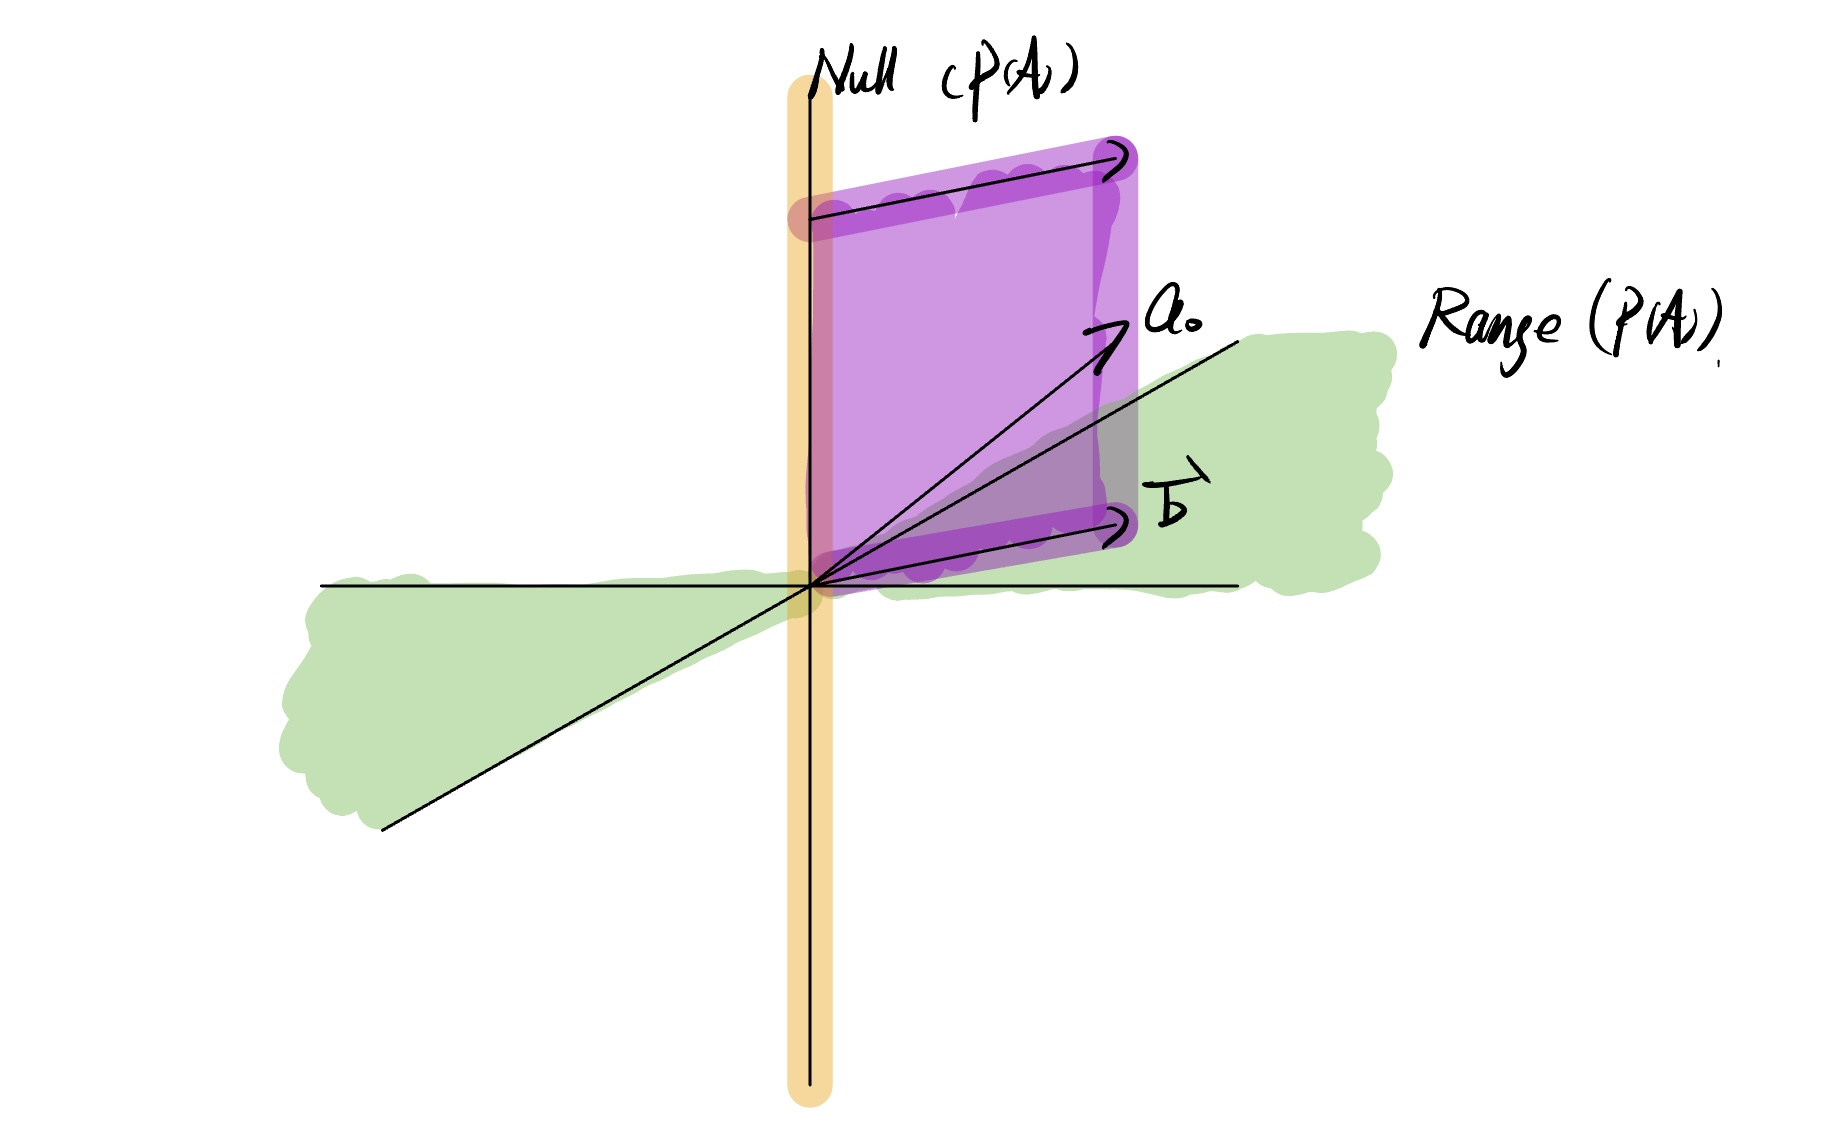
\includegraphics[scale=0.2]{Images/IMG_0291.jpg}
        \caption{My intuition}
    \end{figure}
\end{proof}

\noindent \textbf{Example}:
Solve the non-homogeneous equations.\\
\begin{enumerate}
    \item $a_{n+1}=2a_n+1$
    \item $a_{n+1}=2a_n+3^n$
\end{enumerate}

\noindent\textbf{Answer}:\\
\begin{enumerate}
    \item \begin{itemize}
        \item Let $A$ be the advancement operator. Then we have $$(A-2)\vec{a}=1$$ as the corresponding advancement polynomial equation.
        Let $p(A)=A-2$, first, let's compute $\vec{a_1} \in Null(p(A))$.
        $$(A-2)\vec{a}=0$$
        By the advancement theorem, $a_n=\alpha2^n$. This should be our $\vec{a_1}$.
        \item We only need to find a particular solution, this is usually the hard part.\\
        \underline{One way to do is trying to homogenize it.}
        \begin{equation}
            \begin{cases}
                a_{n+1}-2a_n=1\\
                a_{n+2}-2a_{n+1}=1
            \end{cases}
        \end{equation}
        We use the second equation to minus the first equation:
        $$a_{n+2}-3a_{n+1}+2a_n=0$$
        The corresponding advancement polynomial equation is
        $$(A^2-3A+2)\vec{a}=0$$ $$(A-1)(A-1)\vec{a}=0$$
        By the advancement theorem we have $$a_n=\alpha \cdot 2^n+\beta \cdot 1^n$$
        We notice that $\beta \cdot 1^n$ should be our particular solution $\vec{a_0}$. we should have 
        $$\beta=2\beta+1$$ $$\beta=-1$$
        Therefore, our solution is 
        $$a_n=\alpha \cdot 2^n-1$$
    \end{itemize}
    \item \begin{itemize}
        \item The first part is exactly as the last question, so we have $\vec{a_1}$ which is the sequence $\alpha \cdot 2^n$
        \item I will use two different methods to find the particular solution.
        \begin{enumerate}
            \item \underline{Guess then verify}: Try something that looks a lot like the right hand side.\\
            Guess: $\vec{a_0}$ is the sequence $d \cdot 3^n$.\\
            Solve the polynomial equation $$(A-2)\vec{a_0}=3^n$$ $$d \cdot 3^{n+1}-2 \cdot 3^n=3^n$$ $$3^n(3d-3)=0$$ $$d=1$$
            So $\vec{a_0}$ is the sequence $3^n$
            \item \underline{Trying to homogenize it}: Similar to the last question.\\
            \begin{equation}
                \begin{cases}
                    a_{n+1}-2a_n=3^n\\
                    a_{n+1}-2a_{n+1}=3^{n+1}
                \end{cases}
            \end{equation}
        \end{enumerate}
    \end{itemize}
\end{enumerate}


\section{Generating Functions and Recurrence}
The purpose of a generating function is using a function as a bookkeeping system for a sequence. And we can play the sequence in the continuous world. 
So what is the generating functions look like when we considering the advancement operator?

\begin{theorem}
    Assume the ordinary generating function for $\vec{a}$ is $$F(x)=\sum_{n=0}^{\infty}a_nx^n$$
    Then the ordinary generating function for $A\vec{a}$ is 
    \begin{equation}
        \begin{split}
            \sum_{n=0}^{\infty}a_{n+1}x^n &= \sum_{n=1}^{\infty}a_nx^{n-1}\\
            &= \frac{1}{x} \cdot \sum_{n=1}^{\infty}a_nx^n\\
            &= \frac{1}{x} \cdot (\sum_{n=0}^{\infty}a_nx^n -a_0x^0)\\
            &= \frac{1}{x} \cdot (F(x)-a_0)
        \end{split}
    \end{equation}
\end{theorem}

\begin{theorem}
    Assume the ordinary generating function for $\vec{a}$ is $$F(x)=\sum_{n=0}^{\infty}a_nx^n$$
    Then the ordinary generating function for $A^k\vec{a}$ is 
    \begin{equation}
        \begin{split}
            \sum_{n=0}^{\infty}a_{n+k}x^n &= \sum_{n=k}^{\infty}a_nx^{n-k}\\
            &= \frac{1}{x^k} \cdot \sum_{n=k}^{\infty}a_nx^n\\
            &= \frac{1}{x^k} \cdot (\sum_{n=0}^{\infty}a_nx^n -\sum_{n=0}^{k-1}a_nx^n)\\
            &= \frac{1}{x^k} \cdot (F(x)-\sum_{n=0}^{k-1}a_nx^n)
        \end{split}
    \end{equation}
\end{theorem}

\noindent \textbf{Example}: Suppose $a_n$ is a recurrence that satisfies the equation $$a_{n+3}=5a_{n+1}-a_n+3^n$$
Find a general form for it's ordinary generating function.

\noindent \textbf{Answer}:\\
\begin{equation}
    \begin{split}
        F(x) &= \sum_{n=0}^{\infty}a_nx^n\\
        &= a_0x^0+a_1x^1+a_2x^2+\sum_{n=3}^{\infty}a_nx^n\\
        &= a_0x^0+a_1x^1+a_2x^2+ x^3 (\sum_{n=0}^{\infty}a_{n+3}x^n)\\
        &= a_0x^0+a_1x^1+a_2x^2+ x^3 (5\sum_{n=0}^{\infty}a_{n+1}x^n -\sum_{n=0}^{\infty}a_{n}x^n +\sum_{n=0}^{\infty}3^nx^n)\\
        &= a_0x^0+a_1x^1+a_2x^2+ x^3 (\frac{5}{x}(F(x)-a_0) -F(x) + \frac{1}{1-3x})\\
    \end{split}
\end{equation}
Rearrange the equation above we get $$F(x)= \frac{a_0+a_1x+(a_2-5a_0)x^2}{1-5x^2+x^3} + \frac{x^3}{(1-5x^2+x^3)(1-3x)}$$

\begin{theorem}
    Assume the exponential generating function for $\vec{a}$ is $$f(x)=\sum_{n=0}^{\infty}a_n \frac{x^n}{n!}$$
    Then the exponential generating function for $A\vec{a}$ is $$\sum_{n=0}^{\infty}a_{n+1}\frac{x^n}{n!}=f'(x)$$
\end{theorem}

\noindent \textbf{Remark}:
\begin{itemize}
    \item For ordinary generating functions, we simply need to do algebra.
    \item For exponential generating functions, we need to solve differential equations. (harder!)
\end{itemize}

\noindent \textbf{Example}: Recall, the number of derangements $d_n$ satisfied the recurrence $$d_{n+1}=n \cdot d_n+n \cdot d_{n-1}$$
Find the general form of the exponential generating function $f(x)$ for $d_n$.

\noindent \textbf{Answer}:\\
By definition we have $$f(x)=\sum_{n=0}^{\infty}d_n\frac{x^n}{n!}$$
Consider the derivative of $f(x)$
\begin{equation}
    \begin{split}
        f'(x) &= \sum_{n=0}^{\infty}d_{n+1}\frac{x^n}{n!}\\
        &= \sum_{n=0}^{\infty}nd_n\frac{x^n}{n!}+ \sum_{n=0}^{\infty}nd_{n-1}\frac{x^n}{n!}\\
        &= x \sum_{n=1}^{\infty}d_n\frac{x^{n-1}}{(n-1)!} + x \sum_{n=1}^{\infty}d_{n-1}\frac{x^{n-1}}{(n-1)!}\\
        &= xf'(x)+xf(x)
    \end{split}
\end{equation}
The only thing we need to do is solving the ODE:\\
Rearrange the equation we have
$$(1-x)f'(x)=xf(x)$$ $$\frac{f'(x)}{f(x)}=\frac{x}{1-x}$$
Integrate both sides we have 
$$log(f(x))=-x-log(1-x)+c$$ $$f(x)=\frac{e^{-x+c}}{x-1}$$

\noindent \textbf{Example}\label{cnr}: Suppose $a_n$ satisfies $a_0=a_1=1$ 
and the Catalan recurrence $$a_{n+1}=\sum_{k=0}^{n}a_{n-k}a_k$$
Find the general form of the exponential generating function $F(x)$ for $a_n$.

\noindent \textbf{Answer}:\\
By definition we have $$F(x)=\sum_{n=0}^{\infty}a_n\frac{x^n}{n!}$$
Consider the square of $F(x)$
\begin{equation}
    \begin{split}
        F^2(x) &= \sum_{n=0}^{\infty}(\sum_{k=0}^na_ka_{n-k})x^n\\
        &= \sum_{n=0}^{\infty}a_{n+1}x^n\\
        &= \frac{1}{x} \cdot \sum_{n=0}^{\infty}a_{n+1}x^{n+1}\\
        &= \frac{1}{x} \cdot (\sum_{n=0}^{\infty}a_{n}x^{n} -a_0x^0)\\
        &= \frac{1}{x} \cdot (F(x)-1)
    \end{split}
\end{equation}
Rearrange the equation we have
$$xF^2(x)-F(x)+1=0$$
$$F(X)=\frac{1 \pm \sqrt{1-4x}}{2x}$$
Since $a_0=\lim_{x \to 0}F(x)$, hence we have 
$$F(X)=\frac{1 - \sqrt{1-4x}}{2x}$$
Can use Newton's binomial theorem to compute $$a_n=\frac{1}{n+1}{2n \choose n}$$